\documentclass[border=3pt]{standalone}
% Preâmbulo compartilhado pelos diagramas TikZ da aula
\usepackage[T1]{fontenc}
\usepackage[utf8]{inputenc}
\usepackage{lmodern}
\usepackage{amsmath}
\usepackage{xcolor}
\usepackage{tikz}
\usetikzlibrary{arrows.meta,angles,quotes,decorations.pathmorphing,calc,
                positioning,shapes.geometric,backgrounds,fit}

% Paleta (mesma dos SVGs originais)
\definecolor{dblue}{HTML}{2A5B8C}
\definecolor{dorange}{HTML}{B3541E}
\definecolor{dgreen}{HTML}{4A7C59}
\definecolor{dred}{HTML}{9C4B4B}
\definecolor{dcream}{HTML}{F4F1EA}
\definecolor{dshade}{HTML}{DDD7C9}

% Estilos comuns (prefixo d... para não colidir com chaves internas do pgf)
\tikzset{
  >={Stealth[length=2mm]},
  dguide/.style={gray!55, dashed, line width=0.4pt},
  daxis/.style={gray!60, line width=0.7pt, ->},
  dbody/.style={fill=black!3, draw=black!80, line width=1pt},
  dacc/.style={draw=dblue, line width=1pt},
  dlbl/.style={black!55, font=\small},
  dsub/.style={black!45, font=\footnotesize},
  dstate/.style={circle, draw=black!80, fill=dcream, line width=1pt,
                 minimum size=17mm, font=\large, inner sep=1pt},
  dobs/.style={circle, draw=black!80, fill=dshade, line width=1pt,
               minimum size=14mm, font=\large, inner sep=1pt},
  dbox/.style={rounded corners=2pt, draw=black!80, fill=dcream, line width=1pt,
               align=center, inner sep=6pt},
  dtrans/.style={->, dblue, line width=1pt},
  dmeas/.style={->, dorange, line width=1pt},
}

\begin{document}
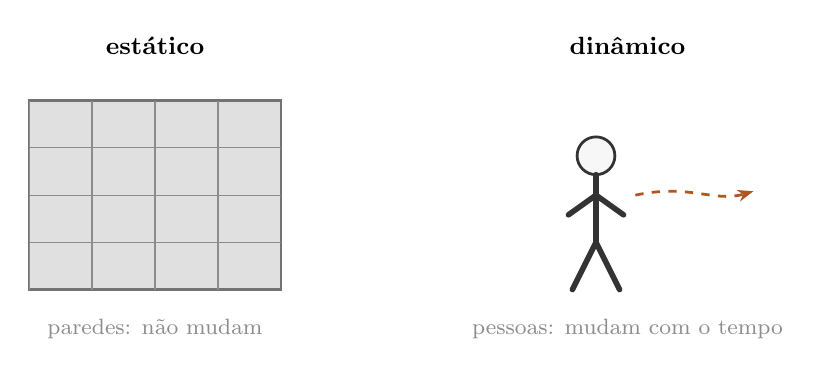
\begin{tikzpicture}[x=1cm,y=1cm]

  % ---- estático: parede ----
  \begin{scope}
    \node[font=\small\bfseries] at (1.6,3.1) {estático};
    \fill[black!12, draw=black!55, line width=1pt] (0,0) rectangle (3.2,2.4);
    \foreach \bx in {0,0.8,1.6,2.4}
      \draw[black!45] (\bx,0) -- (\bx,2.4);
    \foreach \by in {0.6,1.2,1.8}
      \draw[black!45] (0,\by) -- (3.2,\by);
    \node[dsub] at (1.6,-0.5) {paredes: não mudam};
  \end{scope}

  % ---- dinâmico: pessoa em movimento ----
  \begin{scope}[shift={(6,0)}]
    \node[font=\small\bfseries] at (1.6,3.1) {dinâmico};
    % pessoa
    \draw[dbody] (1.2,1.7) circle (0.24);
    \draw[black!80, line width=2pt, line cap=round] (1.2,1.46) -- (1.2,0.6);
    \draw[black!80, line width=2pt, line cap=round] (1.2,1.2) -- (0.85,0.95);
    \draw[black!80, line width=2pt, line cap=round] (1.2,1.2) -- (1.55,0.95);
    \draw[black!80, line width=2pt, line cap=round] (1.2,0.6) -- (0.9,0.0);
    \draw[black!80, line width=2pt, line cap=round] (1.2,0.6) -- (1.5,0.0);
    % movimento
    \draw[->, dorange, line width=1pt, dashed]
      (1.7,1.2) .. controls (2.4,1.35) and (2.7,1.1) .. (3.2,1.25);
    \node[dsub] at (1.6,-0.5) {pessoas: mudam com o tempo};
  \end{scope}

\end{tikzpicture}
\end{document}
